\chapter[Test Driven Development]{Test Driven Development}
  \section{Czym jest TDD?}
    Test Driven Development jest praktyką, według założeń której każda modyfikacja systemu poprzedzona jest stworzeniem odpowiedniego testu opisującego tą modyfikację. Programista zaczyna od napisania testu, który z naturalnych przyczyn (testowany kod nie istnieje a tym etapie) daje wynik negatywny. Następnie napisany zostaje właściwy kod, którego zachowanie zgodne jest z testowanym. Kiedy testy przechodzą można wprowadzić ewentualne poprawki.
    Proces rozwoju oprogramowania w zgodzie z filozofią TDD składa się z wielu takich cyklów, które zobrazować można diagramem:
    
    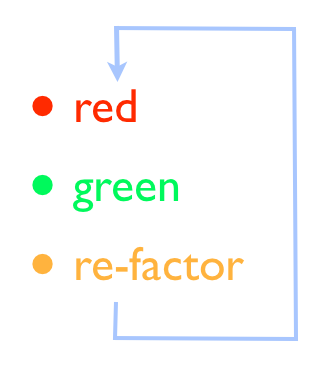
\includegraphics[width=75mm]{images/tdd_red_green_refactor.png}
    
    \begin{description}
      \item[Red] Pierwszy etap cyklu otrzymał swoją nazwę ze względu na to, że w większości środowisk służących do testowania oprogramowania testy, które zakończyły się niepowodzeniem oznaczane są czerwony kolorem. Etap ten polega na napisaniu testu przed rozpoczęciem implementacji właściwej funkcjonalności oraz na uruchomieniu go. Należy upewnić się, że w tym momencie test zakończy się niepowodzeniem - daje to pewność, że faktycznie testujemy nowe zachowanie, którego w tym momencie system jeszcze nie obsługuje, a także że ewentualna przypadkowa modyfikacja tego zachowania zawsze zostanie wykryta przez nieprzechodzący test.
      \item[Green] Drugi etap polega na zaprogramowaniu zachowania opisanego wcześniejszym testem. Programista piszę tylko tyle kodu, aby spełnić warunki testu po czym uruchamia ponownie cały zestaw testów. Uruchomienie tylko ostatniego testu związanego z napisanym kodem jest nie wystarczające - może okazać się, że nasze ostatnie zmiany modyfikują bezpośrednio lub pośrednio wiele obszarów aplikacji. Jak wskazuje nazwa, etap ten powinien zakończyć się gdy wszystkie do tej pory stworzone testy przechodzą pozytywnie.
      \item[Re-factor] Ostatni etap polega na jakościowej modyfikacji kody. W tym momencie programista powinien skupić się na usunięciu wszelkich zbędnych powtórzeń, uproszczeniu implementacji czy też dopracowaniu użytego nazewnictwa zmiennych lub metod. Etap ten nie pociąga za sobą żadnych zmian w sposobie działania oprogramowania, jest jednak równie ważny jak poprzednie, dobry jakościowo kod jest łatwiejszy w utrzymaniu i modyfikacji.
    \end{description}
    
    Opisane powyżej iterację powinny być jak najprostsze. Oznacza to, że każdą implementowaną funkcjonalność należy podzielić na jak najmniejsze części i wykonywać pełen zestaw powyższych kroków dla każdej z nich. Idealna sytuacja to taka, w której pojedynczy test sprawdza tylko jedną rzecz.

  \subsection{Główne zasady TDD}
    \paragraph{Zacznij od testu}
      Test powinien być napisany zanim zacznie się implementacja funkcjonalności. Takie podejście gwarantuje, że będziemy mieli pełen zestaw testów, opisujących każdą funkcję systemu. Inną zaletą jest konieczność dokładnego przemyślenia szczegółów implementacji, jeszcze przed jej rozpoczęciem.
    \paragraph{Zaraz po napisaniu nowe testy powinny dawać negatywny wynik}
      Daje to pewność, że testy faktycznie spełniają swoją funkcję oraz, że każda degradacja funkcjonalności będzie sygnalizowana nieprzechodzącym testem.
      
  \subsection{Przykładowe iteracja TDD}
    Przypuśćmy, że pracujemy nad oprogramowaniem sportowej tablicy wyników. Naszym aktualnym zadaniem jest napisanie metody, która na wejściu otrzymuje nazwy dwóch drużyn sportowych, zwraca zaś łańcuch składający się z nazw tych drużyn połączonych łańcuchem " vs ". Oprogramowanie napisane jest w języku Ruby, do testowania użyjemy biblioteki RSpec.
    
    Praca rozpoczyna się od napisania testu opisującego pożądane zachowanie. W naszym wypadku może on wyglądać tak: 
    
    \begin{verbatim}
      require 'sports_table'

      describe SportsTable do
        it "should properly join team names with 'vs.'" do
          table = SportsTable.new
          table.header('Chicago Bulls', 'Los Angeles Lakers').should == 'Chicago Bulls vs. Los Angeles Lakers'
        end
      end
    \end{verbatim}
    
    Dokładny opis budowy testu zawarty jest w podrozdziale "Narzędzia wspierające TDD dostępne dla języka Ruby" i nie będę go tutaj powielał. Chciałbym jednak zwrócić uwagę na fakt, że już na etapie pisania testu programista zmuszony jest przemyśleć szczegóły implementacji. Zaprezentowany przykład jest bardzo prosty, ale na pierwszy rzut oka widać, że oprócz sprawdzenia poprawności zwracanego wyniku test definiuje także pewne szczegóły architektury programu. Po pierwsze zakładamy, że tablica wyników reprezentowana będzie przez klasę o nazwie \verb+SportsTable+, a żądana funkcjonalność zostanie zaimplementowana jako metoda instancyjna \verb+header+, a więc aby mieć z niej pożytek, użytkownik musi skorzystać z istniejącego obiektu tej klasy. Widać tutaj wyraźnie jedną z głównych zalet testowo zorientowanych metodyk rozwoju oprogramowania - konieczność dokładnego przemyślenia szczegółów implementacji przed jej rozpoczęciem.
    
    Sednem tego konkretnego testu jest jednak upewnienie się, że dla przykładowych danych wejściowych otrzymamy poprawny wynik. W tym wypadku sprawdzamy, czy wywołanie metody \verb+header('Chicago Bulls', 'Los Angeles Lakers')+ na obiekcie klasy \verb+SportsTable+ zwróci łańcuch znaków \verb+Chicago Bulls vs. Los Angeles Lakers+
    
    Po napisaniu uruchamiamy nasz zestaw testów, co kończy się porażką. Zakładając, że rozpoczęliśmy pracę z istniejącą, pustą definicją klasy \verb+SportsTable+ zdefiniowaną w pliku \verb+sports_table.rb+ wynik powinien wyglądać następująco:

    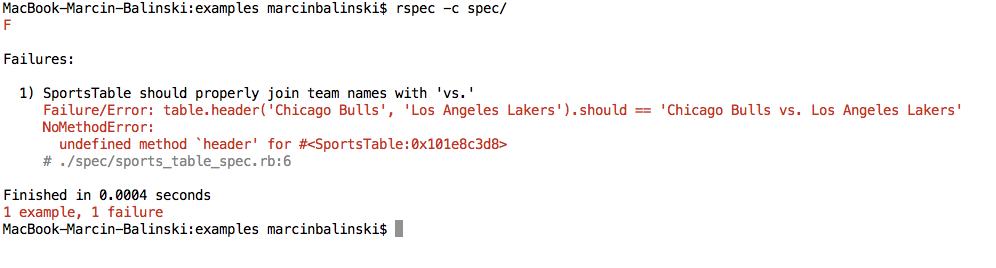
\includegraphics[width=160mm]{images/example1_failure.png}
    
    Tym samym zakończyliśmy pierwszy etap: opisaliśmy wymagane zachowanie testem oraz upewniliśmy się, że test nie przechodzi. Następnym krokiem jest napisanie pierwszej wersji metody \verb+header+:
    
    \begin{verbatim}
      class SportsTable
        def header(team1, team2)
          return team1 + " vs. " + team2
        end
      end
    \end{verbatim}
    
    Ponowne uruchomienie zestawu testów kończy się sukcesem:
    
    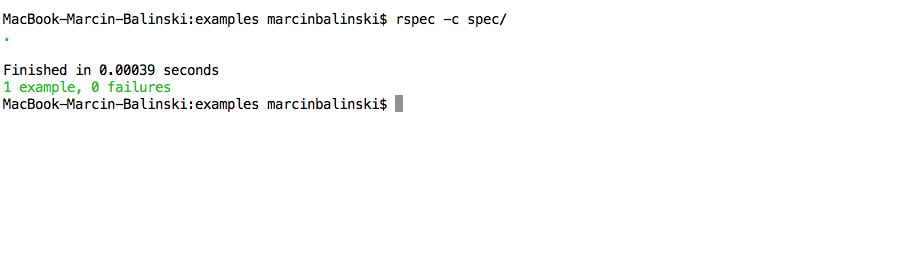
\includegraphics[width=160mm]{images/example1_success.png}
    
    Nasza metoda spełnia wszystkie założenia opisane przez testy, wciąż jednak jest pole do poprawy jakości kodu. W języku Ruby każda metoda domyślnie zwraca ostatnią zdefiniowaną w swoim ciele wartość, możemy więc zrezygnować ze zbędnego słowa kluczowego \verb+return+. Oprócz tego zmienimy sposób konstrukcji wynikowego łańcucha: zrezygnujemy z operatora \verb+++ na rzecz metody \verb+join+ obiektu klasy \verb+Array+. Po modyfikacji metoda \verb+header+ wygląda następująco:
    
    \begin{verbatim}
      class SportsTable
        def header(team1, team2)
          [team1, team2].join(' vs. ')
        end
      end
    \end{verbatim}
    
  Powtórne uruchomienie zestawu testów kończy się sukcesem, a pierwsza iteracja TDD jest zakończona. Zdołaliśmy opisać nową funkcjonalność oraz poprawnie ją zaimplementować. W tym miejscu należy dodać, że w trzecim kroku, po modyfikacji i ulepszeniu kodu nie zmodyfikowaliśmy zestawu testów. W tym konkretnym przypadku nwjważniejszy dla nas jest wynik działania metody \verb+header+, nie zaś szczegóły implementacji. Nie testujemy np. tego, że konstrukcja wynikowego łańcucha znaków odbywa się z użyciem metody \verb+join+. Czasami jednak szczegóły implementacji są równie ważne jak zwracane wynik i wtedy należy napisać odpowiednie testy.
    
  \subsection{Zalety TDD}
    Test Driven Development wymusza na programiście konkretną dyscyplinę pracy. Proces rozwoju oprogramowania jest iteracyjny i bardzo uporządkowany a także wymaga uprzedniego zaplanowania każdej zmiany lub dodatku do istniejącej bazy kodu. Każda iteracja może zostać zakończona jedynie, gdy wszystkie testy zakończą się sukcesem. Taki sposób pracy niesie ze sobą wiele zalet, między innymi:
     
    \begin{itemize}
      \item Pewność, że oprogramowanie zawsze działa zgodnie z założeniami
      \item Wzrost produktywności
      \item Wzrost jakości kodu
      \item Minimalizacja liczby defektów
      \item Możliwość wczesnego wykrycia defektów
      \item Modularyzacja kodu jako pozytywny skutek uboczny
    \end{itemize}

  \section{Narzędzia wspierające TDD dostępne dla języka Ruby}
    
    \subsection{Test::Unit}
      
    \subsection{RSpec}

